\documentclass[10pt,a4paper]{article}

\usepackage[utf8]{inputenc}		% Configuro la codificación
\input{.command.tex}
% En el siguiente archivo se configuran las variables del trabajo práctico
%% \providecommand es similar a \newcommnad, salvo que el primero ante un 
%% conflicto en la compilación, es ignorado.

% Al comienzo de un TP se debe modificar los argumentos de los comandos

\providecommand{\myTitle}{TRABAJO PRÁCTICO 4} 
\providecommand{\mySubtitle}{Banco de filtros}

\providecommand{\mySubject}{Procesamiento de Señales II (86.52)}
\providecommand{\myKeywords}{UBA, Ingeniería, PS2}

\providecommand{\myAuthorSurname}{Anastopulos, Gasparovic, Manso}
\providecommand{\myTimePeriod}{Año 2018 - 2\textsuperscript{do} Cuatrimestre}

% No es necesario modificar este %%%%%%%%%%%%%%
\providecommand{\myHeaderLogo}{header_fiuba}
%%%%%%%%%%%%%%%%%%%%%%%%%%%%%%%%%%%%%%%%%%%%%%%%

% Si se utilizan listings, definir el lenguaje aquí
\providecommand{\myLanguage}{matlab} 
% Crear los integrantes del TP con el comando \PutMember donde
%%		1) Apellido, Nombre
%%		2) Número de Padrón
%%		3) E-Mail
\providecommand{\MembersOnCover}[0]
{		
		\PutMember{Anastópulos, Matías}{95120}{matias.anas@gmail.com}
		\PutMember{Gasparovic, Emiliano}{96123}{emilianit2000@gmail.com}
		\PutMember{Manso, Juan} {96133} {juanmanso@gmail.com}
}

\providecommand{\myGroupNumber}{02}


\Pagebreaktrue		% Setea si hay un salto de página en la carátula
\Indextrue
\Siunitxtrue			% Si quiero utilizar el paquete, \siunixtrue. Si no \siunixfalse
\Todonotestrue		% Habilita/Deshabilita las To-Do Notes y las funciones \unsure, \change, \info, \improvement y \thiswillnotshow.
\Listingstrue
\Keywordsfalse
\Putgrouptrue		% Habilita/Deshabilita el \myGroup en los headers
\Videofalse
				% Archivo con los comandos globales como Título y autores
%Preambulo para articulo científico de LaTeX

\usepackage[a4paper,left=3cm,right=3cm,bottom=3.5cm,top=3.5cm]{geometry} 	% Configuro la geometría del papel
%\usepackage{microtype}								% Mejora el "spacing" de las palabras
\usepackage[spanish]{babel} 							% Compatibilizo los signos del español
	\addto\captionsspanish{\renewcommand{\tablename}{Tabla}}		%% Redefino nombres preestablecidos por Babel
	\addto\captionsspanish{\renewcommand{\listtablename}{Índice de tablas}}	%% y así en vez de Cuadro dirá Tabla.
\usepackage{amsmath, amsfonts, amssymb}						% Entornos matemáticos, fuentes y símbolos
\usepackage{graphicx}								% Necesario para insertar figuras
\usepackage{fancyhdr}								% Para manipular headers y footers
\usepackage[usenames,dvipsnames]{color}						% \color{color deseado} {lo que querés que tenga color}
\usepackage{subcaption}								% Permite captions del tipo 1a, 1b
\usepackage{multirow}								% Para tablas
\usepackage{float}
\usepackage{mathtools}

% Para video
\ifVideo
	\usepackage{media9}
	\addmediapath{./../reportes/}
\fi

%\usepackage{times}
%\usepackage{mathtools}
%\usepackage{upgreek} % letras griegas sin cursiva
%\usepackage{cancel}
\usepackage{rotating}
\usepackage{tikz}
\usepackage{pgfplots}
%	\pgfplotsset{compat=1.12}
	\usetikzlibrary{plotmarks}% matlab2tikz
\usepackage{grffile}% matlab2tikz 
	\usetikzlibrary{calc,patterns,decorations.pathmorphing,decorations.markings}

\ifListings
	\usepackage{listings}

	\providecommand{\lstinputpath}[1]{\lstset{inputpath=#1}}

%	\input{.lst_default.tex}
	\input{.lst_matlab.tex}
%	\input{.lst_c.tex}
%	\input{.lst_c++.tex}
	
% 	\input{.lst_pseudocode.tex}


\fi

\ifSiunitx
\usepackage{siunitx}											% Unidades: \SI {cantidad} {\unidad} (necesita texlive-science)
	\sisetup{load-configurations = abbreviations}							% Habilita poner \cm en vez de \centi\metre
	\sisetup{output-decimal-marker = {,}}									% Cambia los puntos decimales por comas
	\sisetup{per-mode = fraction}											% Pone las unidades como fracción
	\sisetup{quotient-mode = fraction}										
\fi


\ifTodonotes
\usepackage{xargs}
\usepackage[colorinlistoftodos,prependcaption,textsize=tiny]{todonotes}


	\newcommandx{\Juan}[2][1=]{\todo[linecolor=blue,backgroundcolor=blue!25,bordercolor=blue,#1]{#2}}
	\newcommandx{\Mati}[2][1=]{\todo[linecolor=green,backgroundcolor=green!25,bordercolor=green,#1]{#2}} % OliveGreen
	\newcommandx{\Emi}[2][1=]{\todo[linecolor=orange,backgroundcolor=orange!25,bordercolor=orange,#1]{#2}}
	\newcommandx{\unsure}[2][1=]{\todo[linecolor=red,backgroundcolor=red!25,bordercolor=red,#1]{#2}}
	\newcommandx{\thiswillnotshow}[2][1=]{\todo[disable,#1]{#2}}
\fi


\usepackage{booktabs}														% Permite hacer tablas sin separadores en el medio
\usepackage{placeins}														
		\let\Oldsection\section												%% Permite que los flotantes (como figuras) no aparescan
	\renewcommand{\section}{\FloatBarrier\Oldsection}						%% antes o después de su sección correspondiente.
		\let\Oldsubsection\subsection
	\renewcommand{\subsection}{\FloatBarrier\Oldsubsection}		
		\let\Oldsubsubsection\subsubsection
	\renewcommand{\subsubsection}{\FloatBarrier\Oldsubsubsection}
\usepackage{hyperref}														% Debe ser agregado al final del preambulo

\hypersetup
{    bookmarks=true,         % show bookmarks bar?
     unicode=false,          % non-Latin characters in Acrobat’s bookmarks
     pdftoolbar=true,        % show Acrobat’s toolbar?
     pdfmenubar=true,        % show Acrobat’s menu?
     pdffitwindow=false,     % window fit to page when opened
     pdftitle={\myTitle},    		 % title
     pdfauthor={\myAuthorSurname},   % author
	 pdfcreator={\myAuthorSurname},	 % creator = author
     pdfsubject={\mySubject},		 % subject of the document
     pdfkeywords={\myKeywords},
     colorlinks=true,        % false: boxed links; true: colored links
     linkcolor=black,        % color of internal links (change box color with linkbordercolor)
     citecolor=black,        % color of links to bibliography
     filecolor=magenta,      % color of file links
     urlcolor=cyan           % color of external links
}

%Configuro la pagina con los encabezaos y pies de paginas
\pagestyle{fancy}										% Para agregar encabezados y pie de paginas	
\lhead{\mySubject}										% Encabezado izquierdo
\rhead{\includegraphics[scale=0.15]{\myHeaderLogo}} 	% Encabezado derecho (logo de la FIUBA)	
\ifPutgroup
\chead{\texttt{Grupo Nº\myGroupNumber} }%\\ \textit{\footnotesize{\myTimePeriod}}}
\fi				

%% Este archivo contiene las funciones auxiliares para escribir en LaTeX
%% Dichas funciones resuelven la sintaxis de generar figuras, por ejemplo,
%% dejando el código más compacto y facilitando la corrección del mismo.



% Comando para graficar eps. 1er arg, escala. 2do, ruta. 3ro, caption. 4to, label.
\providecommand{\HgraficarEPS}[4]{
			\begin{figure}[h!]
				\centering
					\scalebox{#1}{\input{#2}}
					\caption{#3}
					\label{#4}
			\end{figure}

}

\providecommand{\HgraficarPNG}[4]{
			\begin{figure}[h!]
				\centering
					\includegraphics[scale=#1]{#2}
					\caption{#3}
					\label{#4}
			\end{figure}

}


% Comando para graficar eps en el lugar previsto.
\providecommand{\graficarEPS}[4]{
			\begin{figure}[h]
				\centering
					\scalebox{#1}{\input{#2}}
					\caption{#3}
					\label{#4}
			\end{figure}

}

\providecommand{\graficarPNG}[3]{
			\begin{figure}[h]
				\centering
%					\includegraphics[scale=#1]{#2}
		\includegraphics[width=1.0\textwidth,keepaspectratio]{#1}
					\caption{#2}
					\label{#3}
			\end{figure}

}

\providecommand{\graficarPDF}[3]{
			\begin{figure}[h!]
				\centering
		\includegraphics[width=1.0\textwidth,keepaspectratio]{#1}
					\caption{#2}
					\label{#3}
			\end{figure}

}


\providecommand{\graficarPDFwide}[3]{
			\begin{figure}[h!]
				\centering
		\includegraphics[scale=0.5,trim={6,5cm 0 0 0}]{#1}
					\caption{#2}
					\label{#3}
			\end{figure}

}

\providecommand{\graficarPDFa}[4]{
			\begin{figure}[h!]
				\centering
				\includegraphics[scale=0.5,trim={#1}]{#2}
					\caption{#3}
					\label{#4}
			\end{figure}

}



\providecommand{\underuparrow}[2]{\underset{\underset{#2} \uparrow} #1 }

\providecommand{\cltext}[2]{\color{#1}{\huge{#2}}}

\providecommand{\cstext}[2]{\color{#1}{\large{#2}}}

\providecommand{\vect}[1]{\boldsymbol{#1}}
\providecommand{\dvect}[1]{\dot{\boldsymbol{#1}}}
\providecommand{\dd}{\mathrm{d}}
		% Se proveen un conjunto de funciones extras

% Defino el path de los includegraphics
\graphicspath{{./Figuras/}}		% Directorio que contiene los graficos

% Defino el path para los input de .tex y de .eps
\makeatletter
\def\input@path{{./Figuras/}{./Secciones/}{./Cover_page/}}
\makeatother

% Defino el path del listings
\ifListings
%% Cambiar el nombre de la carpeta si se utilizan Listings
	\lstinputpath{{../Octave/}}
\fi

\definecolor{myred}{rgb}{0.5,0,0}
\definecolor{mygreen}{rgb}{0,0.5,0}

\renewcommand{\thesubsection}{\thesection.\alph{subsection}}

\begin{document}
		% Carátula (formal o simple,_formal o _simple respectivamente) con Resumen
		% incluido e Índice (si es necesario configurar en config.tex) del informe
		\begin{titlepage}
	
		\thispagestyle{empty}

		\begin{center}
			
\includegraphics[scale=0.3]{fiuba}\\
			\large{\textsc{Universidad de Buenos Aires}}\\
			\large{\textsc{Facultad De Ingeniería}}\\
			\small{\myTimePeriod}
		\end{center}

		\vfill

		\begin{center}
			\Large{\underline{\textsc{\mySubject}}}
		\end{center}

		\vfill

		\begin{tabbing}
			\hspace{2cm}\=\+\myTitle\\
				TEMA: \mySubtitle\\
				FECHA: \today\\
			\\
				\MembersHeader
				\MembersOnCover	
		\end{tabbing}

		\begin{abstract}
			El objetivo del presente trabajo es dar una breve exposición acerca de el tema de banco de filtros de reconstrucción perfecta. Se estudiará el uso que se le da a los mismos, junto con el significado de la reconstrucción perfecta en los mismos.

		\end{abstract}

	\ifKeywords
		\begin{center}
			\emph{Palabras Clave: \myKeywords}
		\end{center}
	\fi	

		\vfill
	
\end{titlepage}

\ifPagebreak
	\thispagestyle{empty}
	\ifIndex
		\tableofcontents
%		\listoffigures
%		\listoftables
	\fi

	\pagebreak
\fi


	\setcounter{page}{1}

	\begin{center}{\Large{\textbf{Introducción}}}\end{center}

	
	El sistema a identificar puede verse en la Figura \ref{fig:auto}, se trata de un sistema de amortiguación de un automóvil. 

\vspace*{\fill}
\begin{figure}[H]
\centering
\includegraphics[scale=0.7]{auto.png}
\caption{Sistema Fisico.}
\label{fig:auto} 
\end{figure}
\vspace*{\fill}

	Para identificar el sistema se utiliza el modelo que se observa en la Figura \ref{fig:mbk}. Se trata de un sistema de masa, amortiguador y resorte, donde la entrada $x_{1}$ es el nivel del suelo, y la salida $x_{2}$ es la altura en la que se encuentra el chasis del automóvil. La idea es, mediante un filtro adaptativo, poder estimar las constantes $m$, $b$ y $k$ del sistema.

\vspace*{\fill}
\begin{figure}[H]
\centering
\includegraphics[scale=0.6]{mbk.png}
\caption{Modelo.}
\label{fig:mbk} 
\end{figure}
\vspace*{\fill}

	
	\section{Expansion En Serie De Señales En Tiempo Discreto}
	
	\paragraph{}
En cuanto a expansión en series de señales en tiempo discreto se estudiarán dos tipos, las ortonormales y biortogonales. En todos los casos trabajaremos con señales $x[n] \in l_{2}(\mathbb{Z})$.

% ------------------------------------------------------------------------

\paragraph{Series Ortonormales}
En esta expansión se dispone de una base de funciones $\phi_k$ que satisfacen la condición de ortonormalidad:

\begin{equation}
	\langle \phi_k[n] , \phi_l[n] \rangle = \delta[k - l]
\end{equation}

\paragraph{}
Donde $\delta_[n]$ es la función delta de Kroenecker. Con esta base se puede expresar las señales $x[n]$ de la forma:

\begin{equation}
	x[n] = \sum_{z \in \mathbb{Z}} \langle \phi_k[l] , x[l] \rangle \phi_{k}[n] = \sum_{z \in \mathbb{Z}} X[k] \phi_{k}[n]
\end{equation}

\paragraph{}
Donde:

\begin{equation}
	X[k] = \langle \phi_k[l] , x[l] \rangle = \sum_{l} \phi_{k}^{*} x[l]
\end{equation}

Es la transformada de $x[n]$.

% ------------------------------------------------------------------------

\paragraph{Series Biortogonales}
En este tipo de expansión se dispone, no de una base ortonormal, sino de dos bases $\{ \phi_{k} \}$ y $\{ \tilde{\phi_{k}} \}$, que satisfacen la condición de biortogonalidad:

\begin{equation}
	\langle \phi_k[n] , \tilde{\phi_l}[n] \rangle = \delta[k - l]
\end{equation}

\paragraph{}
Condición que se verá que está relacionada con la construcción perfecta. De esta forma se puede expresar las señales $x[n]$ de la forma:

\begin{equation}
	x[n] = \sum_{z \in \mathbb{Z}} \langle \phi_k[l] , x[l] \rangle \tilde{\phi}_{k}[n] = \sum_{z \in \mathbb{Z}} \tilde{X}[k] \tilde{\phi}_{k}[n]
\end{equation}

\paragraph{}
O de manera equivalente:

\begin{equation}
	x[n] = \sum_{z \in \mathbb{Z}} \langle \tilde{\phi}_k[l] , x[l] \rangle \phi_{k}[n] = \sum_{z \in \mathbb{Z}} X[k] \phi_{k}[n]
\end{equation}

\paragraph{}
Donde:

\begin{equation}
	\tilde{X}[k] = \langle \phi_k[l] , x[l] \rangle
\end{equation}

\paragraph{}
Y:

\begin{equation}
	X[k] = \langle \tilde{\phi}_k[l] , x[l] \rangle
\end{equation}

\paragraph{}
Son las transformadas de $x[n]$, con respecto a las bases $\{ \phi_{k} \}$ y $\{ \tilde{\phi_{k}} \}$.

	
	\section{Bancos De Filtros Para La Implementacion De Dos Ejemplos De Expansion En Series}
	
	\paragraph{}
La idea de esta sección es proponer algunos tipos de expansiones en serie y ver como se podrían implementar utilizando bancos de filtros.

\subsection{Expansión De Haar}

\paragraph{}
La primera de las expansiones será la de Haar, dicha expansión es ortonormal y se basa en la siguiente base de funciones:

\[ \phi_{2k}[n] = \begin{cases} 
      \frac{1}{\sqrt{2}} & n = 2 k, 2 k + 1 \\
      0 & otro \, caso
   \end{cases}
\]

\[ \phi_{2k + 1}[n] = \begin{cases} 
      \frac{1}{\sqrt{2}} & n = 2 k \\
      -\frac{1}{\sqrt{2}} & n = 2 k + 1 \\
      0 & otro \, caso
   \end{cases}
\]

\paragraph{}
La idea sería demostrar que esta expansión puede implementarse con una estructura de bancos de filtros. La estructura a utilizar es la de la figura \ref{fig:banco_de_2}.

	\begin{figure}[h!]
		\centering
		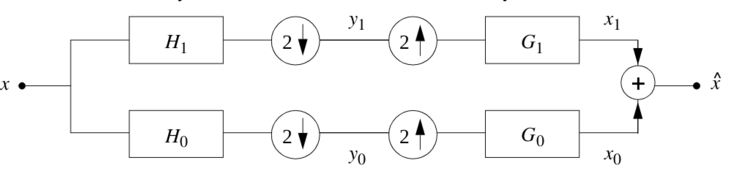
\includegraphics[width=1.0\textwidth, trim = 0cm 0cm 0cm 0cm]{banco_de_2.png}
		\caption{Banco de filtros de dos canales.}
		\label{fig:banco_de_2}
	\end{figure}
	
\paragraph{}
Dicha estructura se compone de una parte de analisis, compuesta por los filtros $H_{0}$ y $H_{1}$, junto con los dos Downsamplers de 2. El objetivo de la parte de analisis es poder computar en las salidas $y_{0}$ e $y_{1}$ los coeficientes de la expansion. La parte de sintesis esta compuesta por los filtros $G_{0}$ y $G_{1}$, junto con los Upsamplers de 2. El objetivo de la parte de sintesis es poder recuperar la señal original a la salida. Si la reconstrucción es perfecta, la salida será una versión posiblemente retrasada de la señal de entrada.

\paragraph{}
Lo primero que se debe ver es que los coeficientes de la expansión se pueden calcular de la siguiente manera:

\begin{equation}
	X[2k] = \langle \phi_{2k} , x \rangle = \frac{1}{\sqrt{2}} (x[2k] + x[2k + 1])
\end{equation}

\begin{equation}
	X[2k + 1] = \langle \phi_{2k + 1} , x \rangle = \frac{1}{\sqrt{2}} (x[2k] - x[2k + 1])
\end{equation}

\paragraph{}
Es decir que los coeficientes pares son el promedio de dos muestras seguidas, y los impares la primera diferencia entre dos muestras seguidas. El siguiente paso es poder elegir los filtros $H$. Si se elige los filtros de la siguiente manera:

\[ h_{0}[n] = \begin{cases} 
      \frac{1}{\sqrt{2}} & n = -1, 0 \\
      0 & otro \, caso
   \end{cases}
\]

\[ h_{1}[n] = \begin{cases} 
      \frac{1}{\sqrt{2}} & n = -1 \\
      -\frac{1}{\sqrt{2}} & n = 0 \\
      0 & otro \, caso
   \end{cases}
\]

\paragraph{}
Los coeficientes se pueden obtener de la siguiente manera:

\begin{equation}
  \left.h_{0}[n] * x[n]\right\vert_{n = 2k} = \sum_{l \in \mathbb{Z}} h_{0}[2k - l] x[l] = \frac{1}{\sqrt{2}} (x[2k] + x[2k + 1]) = X[2k]
\end{equation}

\begin{equation}
  \left.h_{1}[n] * x[n]\right\vert_{n = 2k} = \sum_{l \in \mathbb{Z}} h_{1}[2k - l] x[l] = \frac{1}{\sqrt{2}} (x[2k] - x[2k + 1]) = X[2k + 1]
\end{equation}

\paragraph{}
Observar que evaluar el resultado de la salida del filtro en $2k$ es equivalente a hacer un Downsampling en 2. De esta forma hemos podido computar los coeficientes de la transformación en las salidas $y_{0}$ e $y_{1}$:

\begin{equation}
  y_{0}[k] = X[2k]
\end{equation}

\begin{equation}
  y_{1}[k] = X[2k + 1]
\end{equation}

\paragraph{}
Observar también que las respuestas impulsivas de los filtros son versiones invertidas en el tiempo de las señales de la base:

\begin{equation}
  h_{0}[n] = \phi_{0}[-n]
\end{equation}

\begin{equation}
  h_{1}[n] = \phi_{1}[-n]
\end{equation}

\paragraph{}
En cuanto a la parte de reconstrucción, debemos elegir los filtros $g_{0}$ y $g_{1}$ de forma que la reconstrucción sea perfecta. Se elegirá los filtros de la siguiente manera:

\begin{equation}
  g_{0}[n] = \phi_{0}[n]
\end{equation}

\begin{equation}
  g_{1}[n] = \phi_{1}[n]
\end{equation}

\paragraph{}
Observando que:

\begin{equation}
  \phi_{2k}[n] = g_{0}[n - 2k]
\end{equation}

\begin{equation}
  \phi_{2k + 1}[n] = g_{1}[n - 2k]
\end{equation}

\paragraph{}
Se puede ver que se recupera la señal $x[n]$:

\begin{equation}
  x[n] = \sum_{k \in \mathbb{Z}} X[k] \phi_{k}[n] = \sum_{k \in \mathbb{Z}} y_{0}[k] \phi_{2k}[n] + \sum_{k \in \mathbb{Z}} y_{1}[k] \phi_{2k + 1}[n] = \sum_{k \in \mathbb{Z}} y_{0}[k] g_{0}[n - 2k] + \sum_{k \in \mathbb{Z}} y_{1}[k] g_{1}[n - 2k]
\end{equation}

\paragraph{}
Ver que cada muestra de $y_{i}[k]$ suma una copia de la respuesta impulsiva de $g_{i}[n]$ desplazada en $2k$. Esto puede ser implementado mediante un Upsampling en 2 (Insertando un 0 entre cada dos muestras de $y_{i}[k]$). De esta forma hemos realizado la reconstrucción de la señal utilizando la parte de sintesis del banco de filtros. Con esta elección de los filtros, nuestro banco de filtros de la figura \ref{fig:banco_de_2} es un banco de filtros de reconstrucción perfecta, de dos canales, que implementa la expansión en series de Haar.

\subsection{Expansión Sinc}

El objetivo de la presente sección era poder demostrar la conexión que hay entre los bancos de filtros y las expansiones en serie, incluyendo alguna idea intuitiva de lo que significa reconstrucción perfecta. Si bien este objetivo queda cumplido con la sección anterior, que habla sobre la expansión de Haar, queremos introducir brevemenete la expansión sinc por una cuestión de completitud. La expansión sinc posee cierta dualidad con la expansión de Haar en cierto sentido a exponer. Las funciones base en la expansión de Haar están bien localizadas en el tiempo, ya que se componen de solo dos muestras adyacentes, pero tienen una mala resolución en frecuencia. Las funciones base de la expansión sinc, por el contrario, constituyen las respuestas al impulso de filtros pasabajo y pasaalto ideales. Si bien tienen una resolusión en frecuencia perfecta, tienen una mala localización en el tiempo ya que las respuestas decaen con una proporción de 1/n.

\paragraph{}
Para empezar elegiremos a nuestro $G_{0}$ como un filtro pasabajos ideal:

\[ G_{0}(e^{j\omega}) = \begin{cases} 
      \sqrt{2} & \omega \in [-\frac{\pi}{2}, \frac{\pi}{2}] \\
      0 & \omega \in [\frac{\pi}{2}, \frac{3\pi}{2}]
   \end{cases}
\]

\paragraph{}
Que en el tiempo es:

\begin{equation}
  g_{0}[n] = \frac{1}{\sqrt{2}} \frac{sin \pi n / 2}{\pi n / 2}
\end{equation}

\paragraph{}
Para $G_{1}$ se debe elegir un filtro pasaaltos complementario. Para esto, elegimos una versión modulada de $g_{0}[n]$, invertida en el tiempo, con un desplazamiento en 1 (Por una cuestion de completitud de las funciones base):

\begin{equation}
  g_{1}[n] = (-1)^n g_{0}[-n + 1]
\end{equation}

\paragraph{}
En cuanto a los filtros de analisis $h_{i}[n]$, como en el caso anterior, elegimos una version invertida en el tiempo de los filtros de sintesis $g_{i}[n]$:

\begin{equation}
  h_{i}[n] = g_{i}[-n]
\end{equation}

\paragraph{}
De esta forma hemos construido un banco de filtros que implementa la expansion sinc. La expansion sinc, al igual que la Haar, posee funciones base que son versiones con corrimientos pares de los filtros $g_{i}[n]$:

\begin{equation}
  \phi_{2k}[n] = g_{0}[n - 2k]
\end{equation}

\begin{equation}
  \phi_{2k + 1}[n] = g_{1}[n - 2k]
\end{equation}

	
	\section{Reconstrucción Perfecta}
	
	\paragraph{}
El objetivo de esta sección será aclarar el significado de reconstrucción perfecta. Analizaremos las implicaciones que tiene la reconstrucción perfecta en el dominio del tiempo, en el dominio modulado y en el dominio polifásico. Los análisis serán desarrollados para bancos de filtros de dos canales, pero se darán las fórmulas equivalentes para bancos genéricos de N canales.
\paragraph{}
El significado de reconstrucción perfecta, en el contexto de bancos de filtros, significa que la salida es una version retrasada y posiblemente escalada de la entrada:

\begin{equation}
	\hat{X}(z) = c z^{-k} X(z)
	\label{eq:recons_perf}
\end{equation}

Analizaremos el significado de esta definición en los distintos dominios antes dichos.

\subsection{Análisis en el Dominio del Tiempo}

\Mati{Poner lo que dice de la pagina 130 a 133.}

\begin{equation}
	\begin{pmatrix}
		\vdots \\
		y_0[0] \\
		y_1[0] \\
		y_0[1] \\
		y_1[1] \\
		\vdots \\
	\end{pmatrix}
	=
	\begin{pmatrix}
		\vdots \\
		X[0] \\
		X[1] \\
		X[2] \\
		X[3] \\
		\vdots \\
	\end{pmatrix}
	= T_a 
	\begin{pmatrix}
		\vdots \\
		x[0] \\
		x[1] \\
		x[2] \\
		x[3] \\
		\vdots \\
	\end{pmatrix}
\end{equation}

\begin{equation}
	T_a=
	\begin{bmatrix*}[c]
		\vdots & \vdots & \vdots & & \vdots & \vdots & \vdots\\
		h_0[L-1] & h_0[L-2] & h_0[L-3] & \hdots & h_0[0] & 0 & 0 \\
		h_1[L-1] & h_1[L-2] & h_1[L-3] & \hdots & h_1[0] & 0 & 0 \\
		0 & 0 & h_0[L-1] & \hdots & h_0[2] & h_0[1] & h_0[0] \\
		0 & 0 & h_1[L-1] & \hdots & h_1[2] & h_1[1] & h_1[0] \\
		\vdots & \vdots & \vdots & & \vdots & \vdots & \vdots \\
	\end{bmatrix*}
\end{equation}

Asumiendo que los filtros $h_i$ son FIR de largo $L=2K$, la matriz $T_a$ puede refactorizarse del siguiente modo:

\begin{equation}
	T_a=
	\begin{bmatrix*}[c]
		 & \vdots & \vdots &  & \vdots & \vdots & &\\
		\hdots & A_0 & A_1 & \hdots & A_{K-1} & 0 & \hdots  \\
		\hdots & 0 & A_0 & \hdots & A_{K-2} & A_{K-1} & \hdots  \\
		 & \vdots & \vdots &  & \vdots & \vdots & &\\		
	\end{bmatrix*}
\end{equation}

Siendo cada una de las submatrices $A_i$

\begin{equation}
	A_i=
	\begin{bmatrix*}[c]
		h_0[2K-1-2i] & h_0[2K-2-2i] \\
		h_1[2K-1-2i] & h_1[2K-2-2i] \\
	\end{bmatrix*}
\end{equation}

\subsection{Análisis en el Dominio Modulado}

\Mati{Poner lo que dice de la pagina 134 a 136.}

\subsection{Análisis en el Dominio Polifásico}

	Al igual que en el análisis del dominio modulado, se descompone el sistema periódicamente 
	invariante en varios subsistemas tiempo invariantes. En este caso se descomponen los sistemas en sus componentes polifásicas. 
	Dicha descomposición consta de versiones submuestreadas y con diferentes fases, cuya suma y corrección de fase reconstruye la sucesión inicial.
	%En una trasformación polifásica, se descompone la sucesión en $N$ sucesiones que cada una es retardada $i$ unidades y submuestreada en $N$ con respecto a la original. 
	Formalmente se definen las componentes polifásicas en el tiempo según
		\begin{equation}
			x_i[n] = x[nN+i]
			\label{eq:poly_comp}
		\end{equation}
		
		y en transformada $z$ como 
		\begin{equation} %2.5.20
			X(z)= \sum^{N-1}_{i=0} z^{-i} \, X_i(z^N)
			\label{eq:poly_comp_z}
		\end{equation}
		
		con
		\begin{equation} %2.5.21
			X_i(z)=\sum^{\infty}_{n=-\infty} x[nN+ i]\, z^{-n}
			\label{eq:poly_comp_i_z}
		\end{equation}
%	Formalmente se definen las componentes polifásicas en el tiempo según \eqref{eq:poly_comp} y en transformada $z$ según \eqref{eq:poly_comp_z} con \eqref{eq:poly_comp_i_z}.

	\graficarPNG{polifasico_n_2}{Descomposición polifásica como banco de filtros.}{fig:poli_n_2}
	Se propone probar la reconstrucción perfecta, es decir $x = \hat{x}$ o equivalentemente $X(z) = \hat{X}(z)$. Se presenta el sistema de la Figura \ref{fig:poli_n_2}, considerando $N=2$ y con filtros de análisis $\vect{H}_p(z)$ y síntesis $\vect{G}_p(z)$. 

	Como $N=2$ la transformada $z$ en el dominio polifásico de $x$ resulta:
		\begin{equation}
			X(z) = X_0 (z^2) + z^{-1}\, X_1 (z^2)
			\label{eq:xp_z}
		\end{equation}
	mientras que la componente i-ésima del filtro $H_p$ (calculada al igual que \eqref{eq:poly_comp_z} y \eqref{eq:poly_comp_i_z} salvo la inversión de fase) se simplifica a:
		\begin{equation}
			H_i(z) = H_{i0} (z^2) + z\, H_{i1} (z^2)
			\label{eq:hpi_z}
		\end{equation}

		Así se encuentra $\vect{y}_p(z)$ como:
		\begin{equation}
		\underbrace{\begin{bmatrix} Y_0(z)\\[0.3em] Y_1(z) \end{bmatrix}}_{\vect{y}_p(z)} = \underbrace{\begin{bmatrix} H_{00}(z) & H_{01}(z) \\[0.3em] H_{10}(z) & H_{11}(z) \end{bmatrix}}_{\vect{H}_p(z)} \underbrace{\begin{bmatrix} X_0(z) \\[0.3em] X_1(z) \end{bmatrix}}_{\vect{x}_p(z)}
			\label{eq:in_poly_z}
		\end{equation}

		Del mismo modo, pero en orden inverso al realizar el sobremuestreo primero, se obtiene $\hat{X}(z)$ a partir de $\vect{y}_p(z)$ como:
		\begin{equation}
		\hat{X}(z) = \begin{bmatrix} 1 & z^{-2} \end{bmatrix} \underbrace{\begin{bmatrix} G_{00}(z^2) & G_{01}(z^2) \\[0.3em] G_{10}(z^2) & G_{11}(z^2) \end{bmatrix}}_{\vect{G}_p(z^2)} \underbrace{\begin{bmatrix} Y_0(z^2)\\[0.3em] Y_1(z^2) \end{bmatrix}}_{\vect{y}_p(z^2)} 
			\label{eq:out_poly_z}
		\end{equation}

		Reemplazando \eqref{eq:in_poly_z} en \eqref{eq:out_poly_z}:
		\begin{equation*}
		\hat{X}(z) = \begin{bmatrix} 1 & z^{-2} \end{bmatrix}\; \underbrace{\vect{G}_p(z^2) \; \vect{H}_p(z^2)}_{\vect{T}_p(z^2)} \; \vect{x}_p(z^2)
		\end{equation*}

		Se puede ver que si $\vect{T}_p(z^2) = \vect{I}$, la reconstrucción es perfecta obteniéndose el mismo resultado que \eqref{eq:xp_z}. Para el caso no trivial de la matriz identidad, si la matriz transferencia consta de retardos y factores de amplificación/atenuación, la reconstrucción sigue siendo perfecta como se establece en \eqref{eq:recons_perf}.

	\subsection{Resultados en Bancos de Filtros}
	%\newtheorem{prepo}{Preposición}
	%\theoremstyle{definition}
	El mayor problema de las reconstrucciones es el \emph{aliasing}. Dada la naturaleza de los sistemas periódicamente invariantes, la salida depende no sólo de la entrada sino también de su versión modulada por $(-1)^n$. En términos de la transformada $z$, dependen de $X(z)$ y también de $X(-z)$ imponiendo una distorsión no-harmónica llamada \emph{aliasing}. Por lo tanto, es de gran interés encontrar reconstrucciones libres \emph{aliasing}\\

	%\begin{prepo}
		Se prueba que se puede cancelar el aliasing si sólo si la matriz transferencia $\vect{T}_p(z)$ es seudocirculante. Ésto quiere decir que las filas de la matriz tienen los mismos coeficientes salvo un \emph{shift} lateral, y los coeficientes de la triagular inferior se ven multiplicados por $z$. En $2\times 2$ una matriz de transferencia típica tiene la forma:
		\begin{equation*}
		\vect{T}_p(z) = \begin{bmatrix} F_0 (z) & F_1(z) \\[0.3em] z\, F_1(z) & F_0(z) \end{bmatrix}
		\end{equation*}
			
		Un corolario interesante de la proposicion anterior es que $\vect{T}_p(z)$ tiene que ser una matriz de retardo $d$ seudocirculante. Matemáticamente se ve como:
		\begin{equation*}
		\begin{cases}\vect{T}_p(z)=z^{-k}\begin{bmatrix}1&0\\0&1\end{bmatrix}, &\text{si }d=2k \\[0.5cm]
		\vect{T}_p(z)=z^{-k-1}\begin{bmatrix}0&1\\z&0\end{bmatrix}, &\text{si }d=2k+1\end{cases}
		\end{equation*}
	%\end{prepo}

		Otra preposición que se obtiene es que la reconstrucción es perfecta y sin aliasing si sólo si se hace un submuestreo de tamaño $N$ y $\vect{H}_p(z)$ es de rango $N$ o rango completo (equivalente a pedir que el determinante no sea nulo). La prueba es trivial dado que si se elige a $\vect{G}_p(z)$ como la matriz de cofactores de $\vect{H}_p(z)$, entonces $\vect{T}_p(z) = \det\left(\vect{H}_p(z)\right)\,\vect{I}$ que es seudocirculante.\\

		Un caso interesante es determinar cuándo para filtros FIR la reconstrucción es perfecta. Ésto sucede si solo si el determinante de $\vect{H}_p(z)$ es un retardo puro.\\
		\indent Tomando $\vect{H}_p(z)$ como un retardo puro y $\vect{G}_p(z)$ como la matriz de cofactores de $\vect{H}_p(z)$ se obtiene reconstrucción perfecta con filtros FIR. Por otro lado, si la reconstrucción es perfecta con filtros FIR, $\vect{T}_p(z)$ tiene que ser un retardo puro pseudocirculante: 
		
		\begin{equation*}
			\det(\vect{T}_p(z)) = \det(\vect{G}_p(z)) \det(\vect{H}_p(z)) = z^{-d}
		\end{equation*}
		
		Como $\det(\vect{T}_p(z))$ tiene $d$ polos en 0 y las síntesis $\det(\vect{G}_p(z))$ tiene que tener ceros únicamente (para ser FIR), entonces necesariamente $\det(\vect{H}_p(z)$) no puede tener ceros (excepto en el origen e infinito).\\

	% ESTO SE SACO PARA QUE GIRIBET NO NOS PREGUNTE COSAS MAS AVANZADAS DE ESTO.

		%Por último se destaca el método de QMF (\emph{quadrature mirror filters}) que cancela el \emph{aliasing} en filtros de 2 canales. Como se vio en la sección de dominio modulado para una reconstrucción perfecta libre de \emph{aliasing} se requiere cumplir las Ecuaciones (ecuación 3.2.15 y 16 multiplicada por un delay $z^{-l}$). La solución propuesta entonces se resume en:
		%\begin{equation*}
		%	H^2_0 (z) - H^2_0 (-z) = 2\, z^{-l}
		%\end{equation*}

		%Para el caso particular FIR, ésta condición no se puede satisfacer excepto que se utilice únicamente un filtro de Haar causal. Si se considerasen filtros de fase lineal dicho resultado no se puede obtener pero se puede aproximar.


\Mati{La idea sería dar las formulas equivalentes para N canales. Estan en las páginas 184 a 188.}



	\section{Conclusiones}\label{sec:conclusiones}
		

	A lo largo del trabajo se presentaron herramientas para el entendimiento del concepto de reconstrucción perfecta, partiendo de los ejemplos de las expansiones de Haar y sinc. Tras esa introducción se realizó un análisis más minucioso donde, a partir de los conceptos de ortonormalidad y biortogonalidad, se generaliza para filtros de análisis $\vect{H}(z)$ y síntesis $\vect{G}(z)$. La prueba de la reconstrucción perfecta se realiza bajo los tres dominios: tiempo, modulado y polifásico; obteniéndose la misma solución. Finalmente se demuestra que para que la reconstrucción sea perfecta y libre de \emph{aliasing} el filtro de análisis $\vect{H}(z)$ debe ser lo más transparente posible, representando únicamente un retardo puro (y por consiguiente la transferencia debe ser un \emph{delay} puro).


	% \appendix
\end{document}
